% :Author: Stefan Kottwitz
% :Source: TeXblog - TikZ: shaded cube
%          http://texblog.net/latex-archive/graphics/tikz-cube-3d/
\documentclass{standalone}
\usepackage{tikz}
\usepackage{verbatim}

\begin{comment}

:Title: Sudoku 3D cube
:Tags: 3D, Transformations

This example shows how to create an effective 3D effect using the ``slant`` transformation.
Shading has been added to enhance the 3D impression. Read more about this example over
at TeXblog_. 

.. _TeXblog: http://texblog.net/latex-archive/graphics/tikz-cube-3d/

:Author: Stefan Kottwitz
:Source: `TeXblog - TikZ: shaded cube`__

.. __: http://texblog.net/latex-archive/graphics/tikz-cube-3d/

\end{comment}

\usetikzlibrary{positioning}
\begin{document}
\large
\pagestyle{empty}
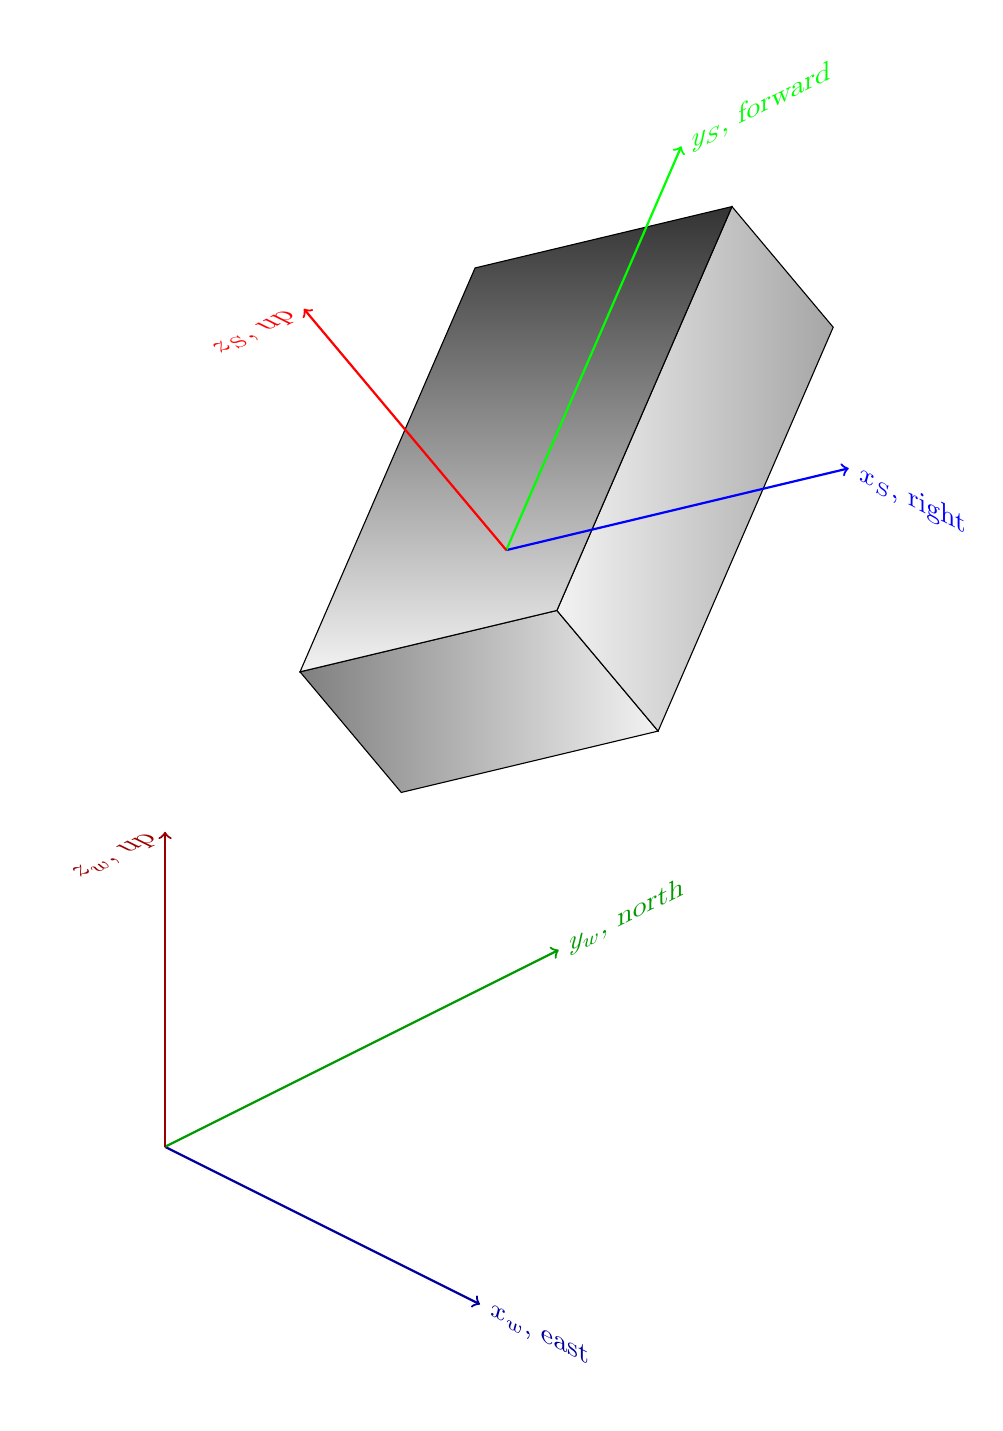
\begin{tikzpicture}[every node/.style={minimum size=1cm},on grid]
\begin{scope}[rotate=40]
\begin{scope}[every node/.append style={yslant=-0.5},yslant=-0.5]
  \shade[right color=gray!10, left color=black!50] (0,0) rectangle (3,2);
  \draw (0,0) rectangle (3,2);
\end{scope}
\begin{scope}[every node/.append style={yslant=0.5},yslant=0.5]
  \shade[right color=gray!70,left color=gray!10] (3,-3) rectangle (8,-1);
  \draw (3,-3) rectangle (8,-1);
\end{scope}
\begin{scope}[every node/.append style={
    yslant=0.5,xslant=-1},yslant=0.5,xslant=-1
  ]
  \shade[bottom color=gray!10, top color=black!80] (7,2) rectangle (2,-1);
  \draw (7,2) rectangle (2,-1);
\end{scope}

%% Axis arrows
\begin{scope}[every node/.append style={yslant=-0.5},yslant=-0.5]
  \draw[blue, thick, ->] (3,3) to (7,3) node[right] {$x_S$, right};
\end{scope}
\begin{scope}[every node/.append style={yslant=0.5},yslant=0.5]
  \draw[green, thick, ->] (3,0) to (8,0) node[right]{$y_S$, forward};
\end{scope}
\begin{scope}[every node/.append style={
    yslant=0.5,xslant=-1},yslant=0.5,xslant=-1
  ]
  \draw[red, thick, ->] (3,0) to (7,4) node[left]{$z_S$, up};
\end{scope}
\end{scope}

\begin{scope}[rotate=0, xshift=-6cm, yshift=-6cm]
\begin{scope}[every node/.append style={yslant=-0.5},yslant=-0.5]
  \draw[blue!60!black, thick, ->] (3,3) to (7,3) node[right] {$x_w$, east};
\end{scope}
\begin{scope}[every node/.append style={yslant=0.5},yslant=0.5]
  \draw[green!60!black, thick, ->] (3,0) to (8,0) node[right]{$y_w$, north};
\end{scope}
\begin{scope}[every node/.append style={
    yslant=0.5,xslant=-1},yslant=0.5,xslant=-1
  ]
  \draw[red!60!black, thick, ->] (3,0) to (7,4) node[left] {$z_w$, up};
\end{scope}
\end{scope}



\end{tikzpicture}
\end{document}